\subsection{Internal closure candidates beyond the theorem stack}

The present manuscript now isolates the cleanest internal upgrade routes instead of leaving them as diffuse future work. They are status-disciplined candidate branches, not proved outputs of the current theorem stack.

\begin{remark}[Axion dark-matter closure route]
The economical internal completion of the existing PQ branch is to identify the
domain-wall number with the same minimal seam class that selects the Higgs branch,
\[
N_{\mathrm{DW}}=1,
\qquad
\theta_i:=\pi(1-\phiz),
\]
and then to close the relic-density block by
\[
\Omega_a h^2
:=
\Delta_R^{-1}
\Bigl[
\Omega_a^{\mathrm{mis}}(f_a,m_a,\theta_i)
+
\Omega_a^{\mathrm{str}}(f_a,N_{\mathrm{DW}})
\Bigr],
\]
where $\Delta_R$ is the scalaron-reheating dilution factor of the same $R^2$
branch that already controls the early-universe dynamics. This keeps both the
initial angle and the entropy dilution internal to the same cosmological block.
\end{remark}

\begin{remark}[Flavored leptogenesis route]
The neutrino block already contains $\nu^c$, $M_R$, $Y_\nu$, and a holonomy phase.
The natural cosmological upgrade is therefore flavored leptogenesis with baryon yield
\[
\eta_B
=
c_{\mathrm{sph}}
\sum_\alpha
\kappa_\alpha\,\varepsilon_{1\alpha},
\]
with flavored CP asymmetries
\[
\varepsilon_{1\alpha}
=
\frac{1}{8\pi (Y_\nu^\dagger Y_\nu)_{11}}
\sum_{j\neq 1}
\Im\!\Bigl[
(Y_\nu^\dagger)_{1\alpha}(Y_\nu)_{\alpha j}(Y_\nu^\dagger Y_\nu)_{1j}
\Bigr]
g(M_j^2/M_1^2).
\]
This keeps baryogenesis inside the same neutrino/family-holonomy architecture
already used for the transport sector instead of importing an unrelated CP source.
\end{remark}

\begin{figure}[t]
\centering
\scriptsize
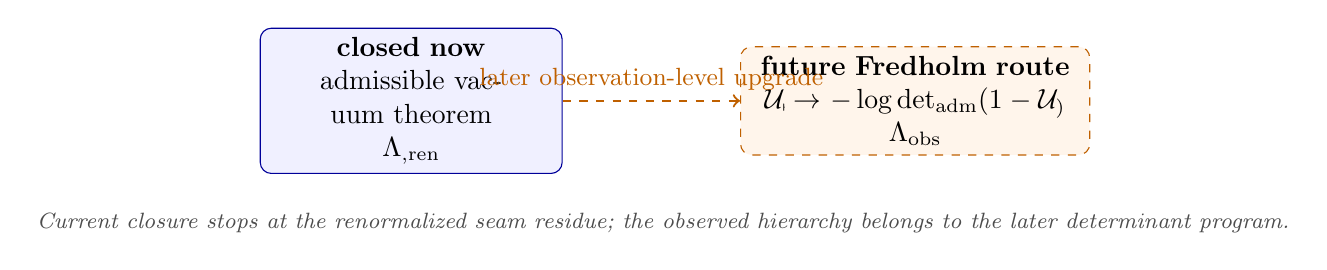
\begin{tikzpicture}[
    closed/.style={draw=blue!60!black, fill=blue!6, rounded corners, text width=3.6cm, minimum height=1.05cm, align=center},
    future/.style={draw=orange!75!black, fill=orange!8, rounded corners, dashed, text width=4.2cm, minimum height=1.2cm, align=center},
    note/.style={font=\footnotesize\itshape, text=black!70, align=center}
]
\node[closed] (now) at (-3.2,0) {\textbf{closed now}\\admissible vacuum theorem\\$\Lambda_{\Seam,\mathrm{ren}}$};
\node[future] (future) at (3.2,0) {\textbf{future Fredholm route}\\$\mathcal U_\Seam \mapsto -\log\det_{\mathrm{adm}}(1-\mathcal U_\Seam)$\\$\Lambda_{\mathrm{obs}}$};
\draw[->, thick, dashed, orange!75!black] (now) -- node[above] {\small later observation-level upgrade} (future);
\node[note] at (0,-1.55) {Current closure stops at the renormalized seam residue; the observed hierarchy belongs to the later determinant program.};
\end{tikzpicture}
\caption{Vacuum-energy status split. The current theorem stack closes only the renormalized seam vacuum energy $\Lambda_{\Seam,\mathrm{ren}}$, while the tiny observed hierarchy is deferred to the later Fredholm-determinant route for $\Lambda_{\mathrm{obs}}$.}
\label{fig:vacuum-energy-status}
\end{figure}

\begin{conjecture}[Seam Fredholm-determinant route for the cosmological constant]
Because TFPT is formulated relatively, bulk zero-point contributions are natural
candidates to cancel in the reference subtraction, leaving only a genuine seam
residue. The corresponding completion route is to define the positive trace-class
seam transfer operator
\[
\mathcal U_\Seam
:=
\Padm\,e^{-\ell_\Seam |B_\Seam|}\,\Padm,
\qquad
\ell_\Seam\,\lambda_1^+(B_\Seam)=S_\Seam,
\qquad
S_\Seam:=\frac{2\pi}{3}\alpha^{-1}(0),
\]
and then set
\[
\Lambda_{\mathrm{obs}}
=
\Mpl^4\Bigl[-\log\det\nolimits_{\mathrm{adm}}(1-\mathcal U_\Seam)\Bigr].
\]
The Fredholm expansion gives
\[
\Lambda_{\mathrm{obs}}
=
\Mpl^4\sum_{k\ge1}\frac{1}{k}\,\tr(\mathcal U_\Seam^k),
\]
so the old seam transseries is recovered as the determinant expansion of one
positive operator. At leading order this gives
\[
\frac{\Lambda_{\mathrm{obs}}}{\Mpl^4}
\approx
\Omega_{\mathrm{adm}}\exp\!\Bigl[-\frac{2\pi}{3}\alpha^{-1}(0)\Bigr]
=
48\,e^{-2\pi\alpha^{-1}(0)/3}
\approx
1.1\times10^{-123}.
\]
This remains a conjectural closure route rather than a proved theorem, but it
turns the tiny cosmological constant into a seam-action effect with controlled
sign and convergence properties instead of a free transseries ansatz.
\end{conjecture}

\appendix

\section{Technical conventions and data layers}
\label{app:tech}

This appendix collects the technical bookkeeping that supports the carrier-first presentation but would slow the early main-text flow if placed before the carrier theorem.

\subsection{Relative objects}

The adjective \enquote{relative} is used in one fixed sense throughout the paper: every operator or action is compared to a declared reference object.

\begin{table}[t]
\centering
\small
\begin{tabularx}{\linewidth}{@{}>{\raggedright\arraybackslash}p{0.22\linewidth}YY@{}}
\toprule
Relative object & Definition or schematic form & Role \\
\midrule
$D_{\mathrm{rel}}$ & $D-D_{\mathrm{ref}}$ or a specified relative pair $(D,D_{\mathrm{ref}})$ & fermionic comparison operator \\
$S_{\mathrm{rel}}$ & $\tr f(D/\Lambda)-\tr f(D_{\mathrm{ref}}/\Lambda)+\frac{i\pi}{2}\Delta\eta$ & relative spectral action \\
$\Ind_{\mathrm{rel}}$ & APS-type index of a relative pair or superconnection package & carrier and bosonic counting \\
$Z_{\mathrm{rel}}$ & $Z_{\mathrm{adm}}[J,\eta,\bar\eta]/Z_{\mathrm{ref}}[0,0,0]$ & normalized admissible generating functional \\
$\Padm$ & $\operatorname*{s-lim}_{\beta\to\infty}e^{-\beta\Kadm}$; factorized form when the elementary projectors commute & operative admissibility selector on the closed branch \\
$\langle W(C)\rangle_{\mathrm{rel}}$ & Wilson observable after subtraction of the declared reference sector & confinement diagnostics \\
$\mathcal H_{\mathrm{rel}}$ & relative Hamiltonian used in admissible-sector minimization & optional record extension \\
\bottomrule
\end{tabularx}
\caption{Conventions on relative objects.}
\label{tab:relative-objects}
\end{table}

\subsection{Layered datum and admissibility}

\begin{construction}[Layered datum]
The technical bookkeeping behind the manuscript uses four levels:
\[
\Tcore
=
\bigl(
\widetilde M\to M,\ \Seam,\ S,\ \Hint,\ \inv,\ D_{\mathrm{rel}},\ f,\ \chiseed
\bigr),
\]
\[
\Tker
=
\bigl(
E_3\oplus E_2,\ Y,\ S^+,\ \gamma,\ B,\ G_{\SM}^{\mathrm{glob}},\ \bone(N_{\mathrm{fam}},N_\Phi)
\bigr),
\]
\[
\Tbridge
=
\bigl(
\mathcal R_{\SM},\ \alpha(0),\ M_Z,\ \{m_c,m_b,m_\tau,m_t\}
\bigr),
\]
\[
\Tcomp
=
\left(
\begin{array}{l}
(\mathsf{Adm},\Kadm,\Padm),\ (\chigeo,\mathcal B_{\mathrm{rel}},\mathbb A_{\Seam}),\ (F,T),\\
(U_6,D_y,\mathcal Y_y^{(\varepsilon)},\epsilon_f),\ (Z_{\mathrm{rel}},\Theta,\Hrel,\Vadm),\\
(\Arec,\Aobs,\Pred)
\end{array}
\right).
\]
\end{construction}

Thus $\Tcore$ is the appendix bookkeeping rewrite of the primitive main-text datum, while $\mathsf{Adm}$ first enters the layered datum only at closure level through $(\mathsf{Adm},\Kadm,\Padm)$.
Equivalently, $\Tprim=(X,S,\Hint,D_{\mathrm{rel}},\inv,f,\chiseed)$ with
$X=\widetilde M\setminus\Seam$, while $\Tcore$ is the expanded bookkeeping form
that keeps the cover map and seam visible.

Conditional horizon and far-downstream E$_8$ data are kept outside this compact layered datum and are introduced only in the dedicated appendix-level extension.

\begin{table}[t]
\centering
\small
\begin{tabularx}{\linewidth}{@{}>{\raggedright\arraybackslash}p{0.12\linewidth}>{\raggedright\arraybackslash}p{0.31\linewidth}>{\raggedright\arraybackslash}p{0.13\linewidth}Y@{}}
\toprule
Level & Objects & Claim role & Function in the present paper \\
\midrule
Core datum & $\widetilde M\to M$, $\Seam$, $S$, $\Hint$, $\inv$, $D_{\mathrm{rel}}$, $f$, $\chiseed$ & Primitive datum & minimal input required to formulate the primitive spectral seed before carrier data and admissibility closure are installed \\
Carrier kernel & $E_3\oplus E_2$, $Y$, $S^+$, $\gamma$, $B$, $G_{\SM}^{\mathrm{glob}}$, $\bone(N_{\mathrm{fam}},N_\Phi)$ & Hard & rigid particle-theory packet extracted from the core datum \\
Closure data & $(\mathsf{Adm},\Kadm,\Padm)$, $(F,T)$, $(\chigeo,\mathcal B_{\mathrm{rel}},\mathbb A_{\Seam})$, $(U_6,D_y,\mathcal Y_y^{(\varepsilon)},\epsilon_f)$, $(Z_{\mathrm{rel}},\Theta,\Hrel,\Vadm)$, $(\Arec,\Aobs,\Pred)$ & Closure & collects the admissibility, family, geometric, transport, OS, record, and vacuum data used by the main closure theorems \\
Benchmark bridge & $\mathcal R_{\SM}$, $\alpha(0)$, $M_Z$, $\{m_c,m_b,m_\tau,m_t\}$ & Benchmark bridge & translates closed compiler outputs into scheme-specified observables \\
\bottomrule
\end{tabularx}
\caption{Core datum versus kernel, closure, and benchmark-bridge structures.}
\label{tab:layered-datum}
\end{table}

\subsection{Symbol guide}

The main text uses a small number of recurrent symbols across different layers. The table below records their first-duty meaning and status class, now including the seam-matching notation introduced in Definition~9.1, so that the manuscript can be read without repeatedly reverse-engineering the bookkeeping.

\begin{table}[t]
\centering
\small
\begin{tabularx}{\linewidth}{@{}>{\raggedright\arraybackslash}p{0.23\linewidth}Y>{\raggedright\arraybackslash}p{0.18\linewidth}@{}}
\toprule
Symbol & First-duty meaning in the paper & Status class \\
\midrule
$\Tprim$ & primitive relative spectral datum $(X,S,\Hint,D_{\mathrm{rel}},\inv,f,\chiseed)$ with $X=\widetilde M\setminus\Seam$; appendix rewrite $\Tcore=(\widetilde M\to M,\Seam,S,\Hint,\inv,D_{\mathrm{rel}},f,\chiseed)$ & Primitive datum \\
$\chiseed$ & primitive seam-even scalar response appearing already in $\Tprim$ and in the primitive spectral seed before geometric reconstruction & Primitive datum \\
$\sigma,\ \chigeo$ & local Weyl field and derived local spectral scale $\chigeo=\Lambda e^\sigma$ on the geometric branch & Closure \\
$\APSdom,\ \APSfam$ & elliptic APS domain for primitive well-posedness and later family-pairing APS data for the imported orbifold--APS theorem & Primitive / closure split \\
$\Tmin$ & reduced theorem-path datum $(\mathcal A,\mathcal H,D,J,\Gamma,\inv,\nu)$ with positive spectral measure $\nu$ & Closure-upgrade route \\
$E_3\oplus E_2$ & minimal carrier split into color and weak sectors & Hard \\
$\bone(N_{\mathrm{fam}},N_\Phi)$ & carrier-side abelian coefficient function before canonical branch evaluation & Hard \\
$\mathsf{Adm},\Kadm,\Padm$ & admissibility predicate, positive constraint operator, and operative selector on the retained branch & Closure \\
$F,\Oadm$ & APS family local system and occupancy count after family closure; $\Oadm$ later feeds the bridge reading of $\deltatop$ & Closure / bridge reinterpretation \\
$\mathcal I_{41}$ & weighted integrity index $10\,\bone=\Omega_{\mathrm{occ}}\gamma+N_\Phi$ on the canonical branch & Closure compression \\
$\delta_{\mathrm{ph}}$ & retained determinant transport saddle on the $C_6$ hexagon & Benchmark bridge \\
$\mathcal R_{\SM}$ & declared map from compiler outputs to scheme-specified observables & Benchmark bridge \\
$\mathcal S_{\mathrm{int}},\mathcal S_{\mathrm{obs}}$ & intrinsic closure surface and observation surface $\mathcal R_{\SM}(\mathcal S_{\mathrm{int}})$ for the compiler interface & Closure / benchmark bridge \\
$\hat m_f,\ m_f^{\mathrm{obs}}$ & internal compiler source masses and their observation-surface images after matching & Closure / benchmark bridge \\
$M_\Sigma,\ g_\Sigma$ & seam matching scale read from the first positive seam boundary mode and the gauge coupling evaluated there & Benchmark bridge \\
$Q_\Theta$ & determinant-sector involution entering admissibility and the projector $P_\Theta$ & Closure \\
$\mathcal C_\Sigma$ & sheet-CP symmetry operator $CP\circ\inv$ on the admissible branch & Closure \\
$T$ & transport generator on the family / holonomy side & Closure \\
$\mathfrak C_\Sigma$ & seam cycle data used by the matching and holonomy packages & Closure / benchmark support \\
$\wspin$ & spin holonomy weight entering the geometric package & Closure \\
$\Arec,\Aobs,\Pred$ & stable record algebra, observer algebra, and prediction map on the admissible sector & Closure \\
\bottomrule
\end{tabularx}
\caption{Symbol guide with first-duty meaning and status class.}
\label{tab:symbol-guide}
\end{table}

\begin{definition}[Admissibility predicate and selector]
In the present paper $\mathsf{Adm}$ denotes a predicate on relative sectors, and $\Padm$ denotes its operator realization on the retained closed branch. We write $\mathsf{Adm}(X)=1$ precisely when:
\begin{enumerate}[label=(\arabic*), leftmargin=1.5em, topsep=3pt, itemsep=2pt]
    \item $X$ lies in the declared domain of the relative operator pair,
    \item the associated relative action or index density is finite after reference subtraction,
    \item the required seam-evenness condition is satisfied,
    \item colored sectors satisfy center neutrality when a hadronic interpretation is intended,
    \item gap-stable transport positivity and the declared closure conditions hold in those sectors used for observable or transport statements.
\end{enumerate}
On those sectors, the selector language and the predicate language are identified by
\[
\mathsf{Adm}(X)=1
\quad\Longleftrightarrow\quad
\Padm X=X.
\]
\end{definition}

\begin{remark}[Operator realization of admissibility]
If one wants an operator language rather than a predicate language, the natural positive generator is $\Kadm$ and its commuting-factor realization is
\[
P_{\mathrm{adm}}=P_{\Seam,+}\,P_{\mathrm{sing}}\,P_{\Theta}\,P_{\mathrm{gap}},
\]
where the factors act on the commuting seam, color, determinant, and transport sectors of the admissible Hilbert-space decomposition. Here $P_{\Seam,+}$ projects to seam-even sectors, $P_{\mathrm{sing}}$ to center-neutral singlets when a hadronic interpretation is intended, $P_{\Theta}$ encodes the declared sheet / determinant selection, and $P_{\mathrm{gap}}$ imposes the transport-side positivity or gap condition. The main text defines $\Padm$ as the zero-temperature projector of $\Kadm$; the appendix records the explicit factorization available on the commuting retained branch.
\end{remark}

\section{Constants atlas and downstream scale grammar}
\label{app:constants}

This appendix collects material that is useful for internal compression but should not dominate the main-text scope of explicit claims.

\subsection{Global rotation angle and constants atlas}

The seam loop is assumed to carry one unit of spectral flow,
\[
U_{\Seam}(\theta)=e^{i\theta},
\qquad
\SF(U_{\Seam})=1,
\qquad
\Delta_{\Seam}=2\pi.
\]
Because the spin lift closes only after $4\pi$, the normalized rotation modulus is
\[
\atheta=\frac{\theta}{4\pi}.
\]
The cascade in \Cref{fig:constant-cascade} is kept here as technical bookkeeping rather than as an early main-text dependency graphic.

\begin{figure}[t]
\centering
\begin{tikzpicture}[
    scale=0.74,
    transform shape,
    >=Latex,
    node distance=1.2cm and 1.0cm,
    box/.style={draw=blue!55!black, rounded corners, fill=blue!4, align=center, minimum width=1.9cm, minimum height=0.95cm},
    hardedge/.style={->, thick},
    bridgeedge/.style={->, dashed, thick},
    definedge/.style={->, dotted, thick},
    optedge/.style={->, dash pattern=on 4pt off 2pt on 1pt off 2pt, thick}
]
\node[box] (theta) {$\theta$};
\node[box, right=of theta] (a) {$\atheta=\theta/(4\pi)$};
\node[box, right=of a] (c3) {$\cthree=1/(8\pi)$};
\node[box, right=of c3] (delta) {$\deltatop=\Oadm \cthree^4$};
\node[box, right=of delta] (phi0) {$\phiz=\phibase+\deltatop$};
\node[box, below=of delta] (phibase) {$\phibase=1/(6\pi)$};
\node[box, below=of phi0] (lambda) {$\lambdaY=\sqrt{\phiz(1-\phiz)}$};
\node[box, below=of c3] (e8) {$\kappa_{E8}$};
\draw[definedge] (theta) -- node[above, font=\scriptsize] {spin lift} (a);
\draw[hardedge] (a) -- node[above, font=\scriptsize] {normalization} (c3);
\draw[bridgeedge] (c3) -- node[above, font=\scriptsize] {transgression} (delta);
\draw[definedge] (phibase) -- node[below right, font=\scriptsize] {base term} (phi0);
\draw[bridgeedge] (delta) -- node[above, font=\scriptsize] {surcharge} (phi0);
\draw[definedge] (phi0) -- node[right, font=\scriptsize] {definition} (lambda);
\draw[optedge] (phi0) -- node[right, font=\scriptsize] {conditional grammar} (e8);
\coordinate (legA) at ($(phibase.south west)+(-0.1,-1.2)$);
\draw[hardedge] (legA) -- ++(0.9,0) node[right, black, font=\scriptsize] {normalization step};
\coordinate (legB) at ($(legA)+(0,-0.55)$);
\draw[bridgeedge] (legB) -- ++(0.9,0) node[right, black, font=\scriptsize] {transgression step};
\coordinate (legC) at ($(legB)+(0,-0.55)$);
\draw[definedge] (legC) -- ++(0.9,0) node[right, black, font=\scriptsize] {declared definition};
\coordinate (legD) at ($(legC)+(0,-0.55)$);
\draw[optedge] (legD) -- ++(0.9,0) node[right, black, font=\scriptsize] {conditional grammar};
\end{tikzpicture}
\caption{Constant cascade used for technical bookkeeping, shown in the occupancy-reinterpretation form for $\deltatop$. Arrow styles encode algebraic role rather than claim status: normalization, transgression, declared definition, and conditional downstream grammar.}
\label{fig:constant-cascade}
\end{figure}

Here the arrow $\atheta\to\cthree$ records a normalization convention internal to the present setup, not an independently proved theorem beyond the declared seam and spin-lift normalization.

\begin{table}[t]
\centering
\scriptsize
\setlength{\tabcolsep}{3pt}
\begin{tabularx}{\linewidth}{@{}>{\raggedright\arraybackslash}p{0.10\linewidth}>{\raggedright\arraybackslash}p{0.18\linewidth}>{\raggedright\arraybackslash}p{0.12\linewidth}>{\raggedright\arraybackslash}p{0.11\linewidth}YY@{}}
\toprule
Symbol & Definition & Compiler role & First origin & Reappears in & Physical meaning \\
\midrule
$\theta$ & seam-loop angle & core datum & seam data & $\atheta$ & geometric rotation variable \\
$\atheta$ & $\theta/(4\pi)$ & hard normalization & spin lift & $\cthree$, phase grammar & normalized cover rotation \\
$\cthree$ & $1/(8\pi)$ & hard kernel constant & seam normalization & $\deltatop$, $\beta$, $\sigma$ & seam normalization constant \\
$\phibase$ & $1/(6\pi)$ & hard kernel constant & carrier geometry & $\phiz$ & base opening \\
$\deltatop$ & $\frac{3}{256\pi^4}$; bridge reading $\Oadm\cthree^4$ & hard kernel value with bridge occupancy reinterpretation & retained numerical kernel & $\phiz$, $\delta_2$ & topological surcharge \\
$\phiz$ & $\frac{1}{6\pi}+\frac{3}{256\pi^4}$ & retained canonical seed & retained numerical kernel & $\lambdaY$, $\beta$, flavor & minimal nontrivial opening \\
$\gamma$ & $\tr_EY^2=5/6$ & hard kernel invariant & carrier packet & $\kappa_{E8}$, $\delta_2$ & carrier norm \\
$B$ & $\rank E_3/\rank E_2=3/2$ & hard kernel invariant & carrier packet & $\delta_2$ & carrier rank ratio \\
$\Oadm$ & $3\times16=48$ & closure quantity with bridge reinterpretation & APS family closure & $\deltatop$ & admissible chiral-state count on the family-closed branch \\
$\bone$ & $\frac43N_{\mathrm{fam}}+\frac1{10}N_\Phi$ & hard kernel output & abelian index & benchmark map & hypercharge trace coefficient \\
$\kappa_{E8}$ & $\gamma/\ln(248/60)$ & conditional grammar & Appendix~\ref{app:constants} & scale ladder & optional scale spacing \\
\bottomrule
\end{tabularx}
\caption{Constants atlas for the present manuscript.}
\label{tab:constants-atlas}
\end{table}

